\newpage
\section{Results}
\label{S4}


/{Describe the results. Graphs and tables shall be commented in text. To facilitate the comparison of the results for different design solutions, include several reliability graphs in one diagram.}/
\begin{table}[h]
\centering
\begin{tabular}{| c | c | c | c |}
\hline
\multicolumn{2}{|c|}{Units} & Distributed & Centralized\\
\hline
\multirow{2}{*}{Wheel Unit Subsystem Full Functionality} & Reliability & 0.7450 & 0.8357\\
 & MTTF & 3.93  & 5.52\\
\hline
\multirow{2}{*}{Wheel Unit Subsystem Degraded Functionality}& Reliability & 0.9726  & 0.9891\\
 & MTTF & 7.24 & 10.2\\
\hline
\multirow{2}{*}{Central Unit}& Reliability& 0.9806  & 0.9952\\
 & MTTF & 21.3  & 20.8\\
\hline
\multirow{2}{*}{Entire System Full Functionality}& Reliability & 0.7305  & 0.8316\\
 & MTTF & 3.74 & 5.23\\
\hline
\multirow{2}{*}{Entire System Degraded Functionality}& Reliability & 0.9537 & 0.9843\\
 & MTTF & 6.56 & 9.06\\
\hline
\end{tabular}
\caption{Reliability and MTTF results}
\label{tab:Put a Lable}
\end{table}
\\/{Insert Reliability Graphs and comment them in the text. Make sure that the caption numbers are correct.}/

\begin{figure}[H]
  \centering
  % GNUPLOT: LaTeX picture
  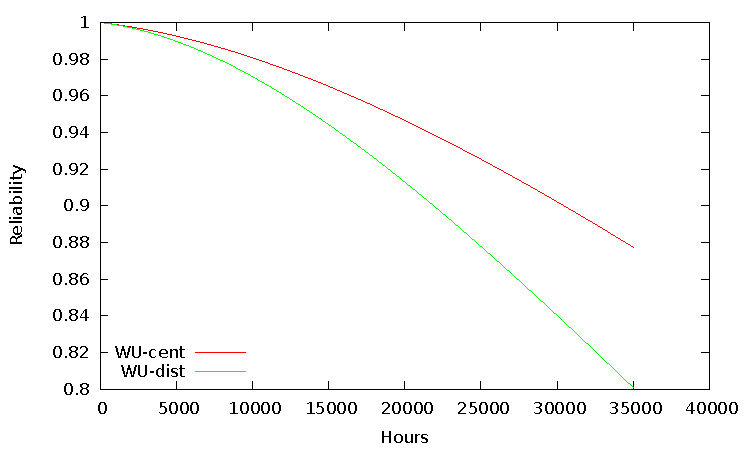
\includegraphics{plots/WU.pdf}
  \caption{One Wheel Unit}
  \label{fig:wu}
\end{figure}
\begin{figure}[H]
  \centering
  % GNUPLOT: LaTeX picture
  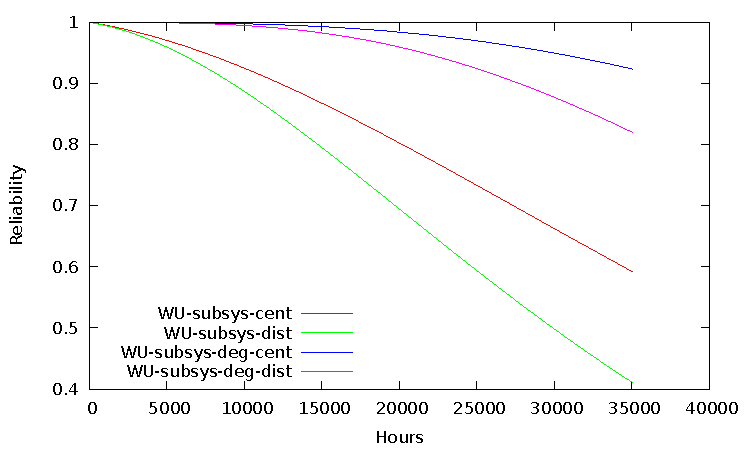
\includegraphics{plots/WUs.pdf}
  \caption{Wheel Units}
  \label{fig:wus}
\end{figure}
\begin{figure}[H]
  \centering
  % GNUPLOT: LaTeX picture
  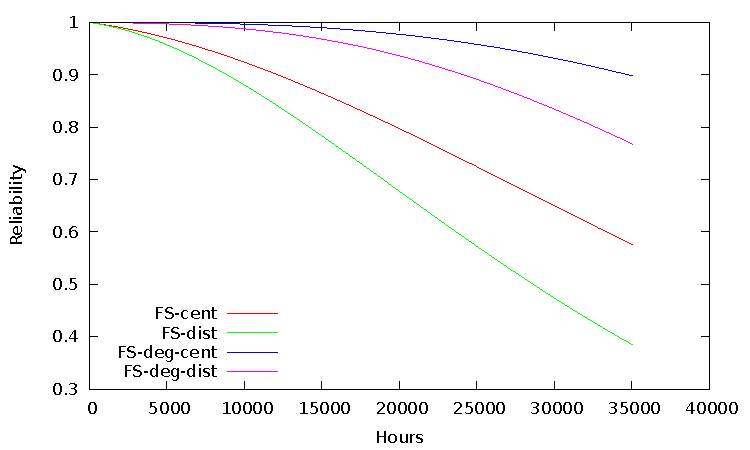
\includegraphics{plots/FS.pdf}
  \caption{Full system}
  \label{fig:fs}
\end{figure}
\begin{figure}[H]
  \centering
  % GNUPLOT: LaTeX picture
  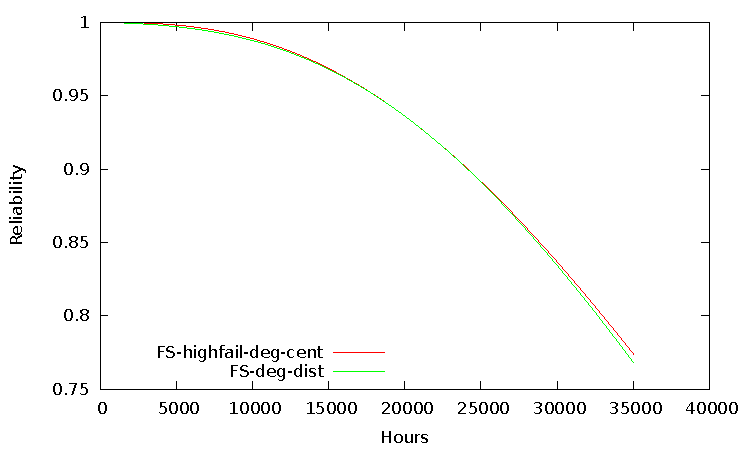
\includegraphics{plots/FS-hf.pdf}
  \caption{Full system in degraded mode with higher fail rate}
  \label{fig:cfs_hf}
\end{figure}
\begin{figure}[H]
  \centering
  % GNUPLOT: LaTeX picture
  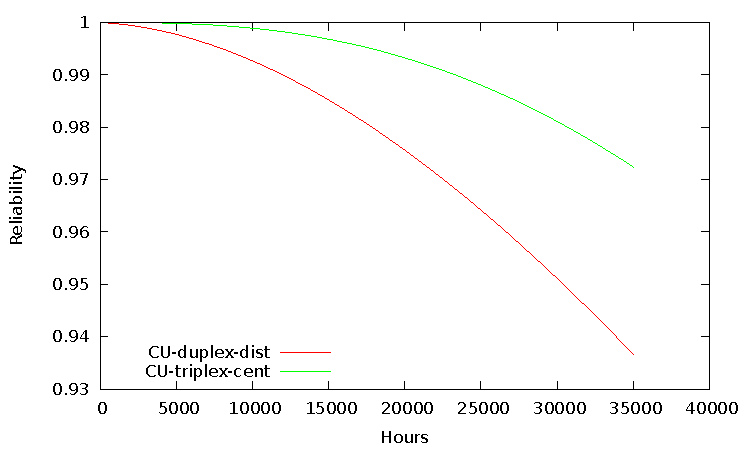
\includegraphics{plots/CUs.pdf}
  \caption{cu}
  \label{fig:cu}
\end{figure}